\section*{Questão 2}

\paragraph{} O mesmo algoritmo da questão anterior é rodado
desta vez com n = m - 1 = 16. Nessas condições devemos ter como 
resposta o polinômio interpolador. Os coeficientes são mostrados
 na tabela \ref{tab:quest2-X16}.
O erro quadrático médio encontrado foi:

\begin{displaymath}
	E_{rms_{16}} = 0.008
\end{displaymath}

\paragraph{} O polinômio é plotado em \ref{fig:quest2} e em \ref{fig:quest2-zoom} 
limitamos o eixo y para observarmos melhor o comportamento da função.
Os gráfico nos mostram que, como esperávamos, o ajuste polinomial
para n = m-1 bate perfeitamente com os pontos considerados. O erro rms calculado
não é exatamente 0 como esperávamos mas isso pode ser devido a erros de truncamento
que ocorrem durante o processo. 
 Se fossemos usar o mesmo critério utilizado na
questão 1 
para escolher o melhor ajuste teríamos que o polinômio interpolador fornece de longe
o melhor ajuste para os dados. No entanto, as altas inclinações da curva entre
os pontos tabelados e as altíssimas inclinações perto
dos extremos geram dúvidas quanto a aplicação do polinômio para
pontos fora aqueles que já tínhamos tabelados. Novamente, não conhecendo o que os 
dados devem representar não se pode decidir se o comportamento esperado corresponde
ao encontrado.

\paragraph{}Nas aplicações mais comuns espera-se que uma função f(t) esteja próxima
de $f(t_0)$ quando t está próximo de $t_0$. O polinômio interpolador não apresenta 
essa propriedade, ele é contínuo mas possui altas derivadas em quase todos os pontos.
Por exemplo, se t está entre $t_1$ e $t_2$ pode ser esperado que y(t) esteja
entre $y_1$ ou $y_2$ ou ainda que tenha ao menos magnitude comparável com estes. 
O gráfico nos mostra que no polinômio interpolador para um t nesse intervalo f pode assumir
valores cerca de 1000 vezes o máximo de f em todos os $t_i$'s conhecidos. Para a maioria
das aplicações este não é o comportamento esperado. 

\paragraph{}A primeira questão nos  mostrou que o ajuste linear nos dá
o menor erro quadrático médio dentre os graus tomados e até aqui vemos que
o polinômio interpolador nos dá uma grande variação em um intervalo pequeno.
Escolhemos portanto o ajuste linear como o mais adequado para descrever os dados da tabela.
\FloatBarrier
\begin{figure}[!htp]
	\begin{subfigure}[!htp]{0.5\textwidth}
	% GNUPLOT: LaTeX picture with Postscript
\begingroup
  \fontfamily{phv}%
  \selectfont
\definecolor{t}{rgb}{0.5,0.5,0.5}
  \makeatletter
  \providecommand\color[2][]{%
    \GenericError{(gnuplot) \space\space\space\@spaces}{%
      Package color not loaded in conjunction with
      terminal option `colourtext'%
    }{See the gnuplot documentation for explanation.%
    }{Either use 'blacktext' in gnuplot or load the package
      color.sty in LaTeX.}%
    \renewcommand\color[2][]{}%
  }%
  \providecommand\includegraphics[2][]{%
    \GenericError{(gnuplot) \space\space\space\@spaces}{%
      Package graphicx or graphics not loaded%
    }{See the gnuplot documentation for explanation.%
    }{The gnuplot epslatex terminal needs graphicx.sty or graphics.sty.}%
    \renewcommand\includegraphics[2][]{}%
  }%
  \providecommand\rotatebox[2]{#2}%
  \@ifundefined{ifGPcolor}{%
    \newif\ifGPcolor
    \GPcolortrue
  }{}%
  \@ifundefined{ifGPblacktext}{%
    \newif\ifGPblacktext
    \GPblacktextfalse
  }{}%
  % define a \g@addto@macro without @ in the name:
  \let\gplgaddtomacro\g@addto@macro
  % define empty templates for all commands taking text:
  \gdef\gplbacktext{}%
  \gdef\gplfronttext{}%
  \makeatother
  \ifGPblacktext
    % no textcolor at all
    \def\colorrgb#1{}%
    \def\colorgray#1{}%
  \else
    % gray or color?
    \ifGPcolor
      \def\colorrgb#1{\color[rgb]{#1}}%
      \def\colorgray#1{\color[gray]{#1}}%
      \expandafter\def\csname LTw\endcsname{\color{white}}%
      \expandafter\def\csname LTb\endcsname{\color{black}}%
      \expandafter\def\csname LTa\endcsname{\color{black}}%
      \expandafter\def\csname LT0\endcsname{\color[rgb]{1,0,0}}%
      \expandafter\def\csname LT1\endcsname{\color[rgb]{0,1,0}}%
      \expandafter\def\csname LT2\endcsname{\color[rgb]{0,0,1}}%
      \expandafter\def\csname LT3\endcsname{\color[rgb]{1,0,1}}%
      \expandafter\def\csname LT4\endcsname{\color[rgb]{0,1,1}}%
      \expandafter\def\csname LT5\endcsname{\color[rgb]{1,1,0}}%
      \expandafter\def\csname LT6\endcsname{\color[rgb]{0,0,0}}%
      \expandafter\def\csname LT7\endcsname{\color[rgb]{1,0.3,0}}%
      \expandafter\def\csname LT8\endcsname{\color[rgb]{0.5,0.5,0.5}}%
    \else
      % gray
      \def\colorrgb#1{\color{black}}%
      \def\colorgray#1{\color[gray]{#1}}%
      \expandafter\def\csname LTw\endcsname{\color{white}}%
      \expandafter\def\csname LTb\endcsname{\color{black}}%
      \expandafter\def\csname LTa\endcsname{\color{black}}%
      \expandafter\def\csname LT0\endcsname{\color{black}}%
      \expandafter\def\csname LT1\endcsname{\color{black}}%
      \expandafter\def\csname LT2\endcsname{\color{black}}%
      \expandafter\def\csname LT3\endcsname{\color{black}}%
      \expandafter\def\csname LT4\endcsname{\color{black}}%
      \expandafter\def\csname LT5\endcsname{\color{black}}%
      \expandafter\def\csname LT6\endcsname{\color{black}}%
      \expandafter\def\csname LT7\endcsname{\color{black}}%
      \expandafter\def\csname LT8\endcsname{\color{black}}%
    \fi
  \fi
  \setlength{\unitlength}{0.0500bp}%
  \begin{picture}(7936.00,5668.00)%
    \gplgaddtomacro\gplbacktext{%
      \csname LTb\endcsname%
      \put(882,1116){\makebox(0,0)[r]{\strut{}-1400}}%
      \put(882,1617){\makebox(0,0)[r]{\strut{}-1200}}%
      \put(882,2119){\makebox(0,0)[r]{\strut{}-1000}}%
      \put(882,2620){\makebox(0,0)[r]{\strut{}-800}}%
      \put(882,3121){\makebox(0,0)[r]{\strut{}-600}}%
      \put(882,3623){\makebox(0,0)[r]{\strut{}-400}}%
      \put(882,4124){\makebox(0,0)[r]{\strut{}-200}}%
      \put(882,4626){\makebox(0,0)[r]{\strut{} 0}}%
      \put(882,5127){\makebox(0,0)[r]{\strut{} 200}}%
      \put(990,936){\makebox(0,0){\strut{} 0}}%
      \put(1726,936){\makebox(0,0){\strut{} 0.2}}%
      \put(2461,936){\makebox(0,0){\strut{} 0.4}}%
      \put(3197,936){\makebox(0,0){\strut{} 0.6}}%
      \put(3933,936){\makebox(0,0){\strut{} 0.8}}%
      \put(4668,936){\makebox(0,0){\strut{} 1}}%
      \put(5404,936){\makebox(0,0){\strut{} 1.2}}%
      \put(6140,936){\makebox(0,0){\strut{} 1.4}}%
      \put(6875,936){\makebox(0,0){\strut{} 1.6}}%
      \put(7611,936){\makebox(0,0){\strut{} 1.8}}%
      \put(144,3121){\makebox(0,0){\strut{}y(t)}}%
      \put(4300,666){\makebox(0,0){\strut{}t}}%
      \put(4300,5397){\makebox(0,0){\strut{}Ajuste Polinomial}}%
    }%
    \gplgaddtomacro\gplfronttext{%
      \csname LTb\endcsname%
      \put(4539,333){\makebox(0,0)[r]{\strut{}$y_{16}(t)$}}%
      \csname LTb\endcsname%
      \put(4539,153){\makebox(0,0)[r]{\strut{}data points}}%
    }%
    \gplbacktext
    \put(0,0){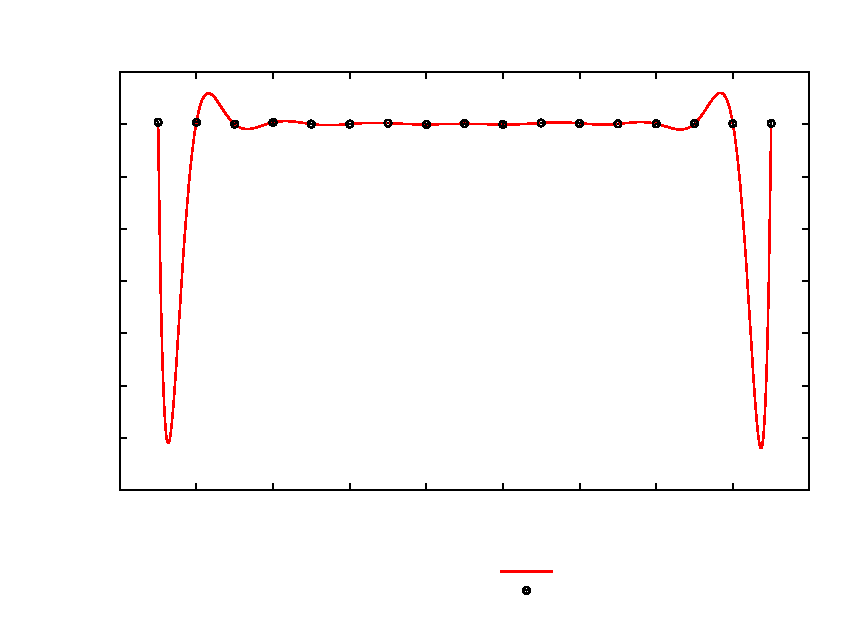
\includegraphics{./../LaTeX/graph/quest2}}%
    \gplfronttext
  \end{picture}%
\endgroup

	\caption{Polinômio interpolador(fitting polinomial de grau 16 = m - 1}
	\label{fig:quest2}
	\end{subfigure}

	\begin{subfigure}[!htp]{0.5\textwidth}
	% GNUPLOT: LaTeX picture with Postscript
\begingroup
  \fontfamily{phv}%
  \selectfont
\definecolor{t}{rgb}{0.5,0.5,0.5}
  \makeatletter
  \providecommand\color[2][]{%
    \GenericError{(gnuplot) \space\space\space\@spaces}{%
      Package color not loaded in conjunction with
      terminal option `colourtext'%
    }{See the gnuplot documentation for explanation.%
    }{Either use 'blacktext' in gnuplot or load the package
      color.sty in LaTeX.}%
    \renewcommand\color[2][]{}%
  }%
  \providecommand\includegraphics[2][]{%
    \GenericError{(gnuplot) \space\space\space\@spaces}{%
      Package graphicx or graphics not loaded%
    }{See the gnuplot documentation for explanation.%
    }{The gnuplot epslatex terminal needs graphicx.sty or graphics.sty.}%
    \renewcommand\includegraphics[2][]{}%
  }%
  \providecommand\rotatebox[2]{#2}%
  \@ifundefined{ifGPcolor}{%
    \newif\ifGPcolor
    \GPcolortrue
  }{}%
  \@ifundefined{ifGPblacktext}{%
    \newif\ifGPblacktext
    \GPblacktextfalse
  }{}%
  % define a \g@addto@macro without @ in the name:
  \let\gplgaddtomacro\g@addto@macro
  % define empty templates for all commands taking text:
  \gdef\gplbacktext{}%
  \gdef\gplfronttext{}%
  \makeatother
  \ifGPblacktext
    % no textcolor at all
    \def\colorrgb#1{}%
    \def\colorgray#1{}%
  \else
    % gray or color?
    \ifGPcolor
      \def\colorrgb#1{\color[rgb]{#1}}%
      \def\colorgray#1{\color[gray]{#1}}%
      \expandafter\def\csname LTw\endcsname{\color{white}}%
      \expandafter\def\csname LTb\endcsname{\color{black}}%
      \expandafter\def\csname LTa\endcsname{\color{black}}%
      \expandafter\def\csname LT0\endcsname{\color[rgb]{1,0,0}}%
      \expandafter\def\csname LT1\endcsname{\color[rgb]{0,1,0}}%
      \expandafter\def\csname LT2\endcsname{\color[rgb]{0,0,1}}%
      \expandafter\def\csname LT3\endcsname{\color[rgb]{1,0,1}}%
      \expandafter\def\csname LT4\endcsname{\color[rgb]{0,1,1}}%
      \expandafter\def\csname LT5\endcsname{\color[rgb]{1,1,0}}%
      \expandafter\def\csname LT6\endcsname{\color[rgb]{0,0,0}}%
      \expandafter\def\csname LT7\endcsname{\color[rgb]{1,0.3,0}}%
      \expandafter\def\csname LT8\endcsname{\color[rgb]{0.5,0.5,0.5}}%
    \else
      % gray
      \def\colorrgb#1{\color{black}}%
      \def\colorgray#1{\color[gray]{#1}}%
      \expandafter\def\csname LTw\endcsname{\color{white}}%
      \expandafter\def\csname LTb\endcsname{\color{black}}%
      \expandafter\def\csname LTa\endcsname{\color{black}}%
      \expandafter\def\csname LT0\endcsname{\color{black}}%
      \expandafter\def\csname LT1\endcsname{\color{black}}%
      \expandafter\def\csname LT2\endcsname{\color{black}}%
      \expandafter\def\csname LT3\endcsname{\color{black}}%
      \expandafter\def\csname LT4\endcsname{\color{black}}%
      \expandafter\def\csname LT5\endcsname{\color{black}}%
      \expandafter\def\csname LT6\endcsname{\color{black}}%
      \expandafter\def\csname LT7\endcsname{\color{black}}%
      \expandafter\def\csname LT8\endcsname{\color{black}}%
    \fi
  \fi
  \setlength{\unitlength}{0.0500bp}%
  \begin{picture}(7936.00,5668.00)%
    \gplgaddtomacro\gplbacktext{%
      \csname LTb\endcsname%
      \put(666,1116){\makebox(0,0)[r]{\strut{} 0}}%
      \put(666,1785){\makebox(0,0)[r]{\strut{} 2}}%
      \put(666,2453){\makebox(0,0)[r]{\strut{} 4}}%
      \put(666,3122){\makebox(0,0)[r]{\strut{} 6}}%
      \put(666,3790){\makebox(0,0)[r]{\strut{} 8}}%
      \put(666,4459){\makebox(0,0)[r]{\strut{} 10}}%
      \put(666,5127){\makebox(0,0)[r]{\strut{} 12}}%
      \put(774,936){\makebox(0,0){\strut{} 0}}%
      \put(1534,936){\makebox(0,0){\strut{} 0.2}}%
      \put(2293,936){\makebox(0,0){\strut{} 0.4}}%
      \put(3053,936){\makebox(0,0){\strut{} 0.6}}%
      \put(3813,936){\makebox(0,0){\strut{} 0.8}}%
      \put(4572,936){\makebox(0,0){\strut{} 1}}%
      \put(5332,936){\makebox(0,0){\strut{} 1.2}}%
      \put(6092,936){\makebox(0,0){\strut{} 1.4}}%
      \put(6851,936){\makebox(0,0){\strut{} 1.6}}%
      \put(7611,936){\makebox(0,0){\strut{} 1.8}}%
      \put(144,3121){\makebox(0,0){\strut{}y(t)}}%
      \put(4192,666){\makebox(0,0){\strut{}t}}%
      \put(4192,5397){\makebox(0,0){\strut{}Fitting Polinomial várias ordens}}%
    }%
    \gplgaddtomacro\gplfronttext{%
      \csname LTb\endcsname%
      \put(4431,333){\makebox(0,0)[r]{\strut{}$y_{16}(t)$}}%
      \csname LTb\endcsname%
      \put(4431,153){\makebox(0,0)[r]{\strut{}data points}}%
    }%
    \gplbacktext
    \put(0,0){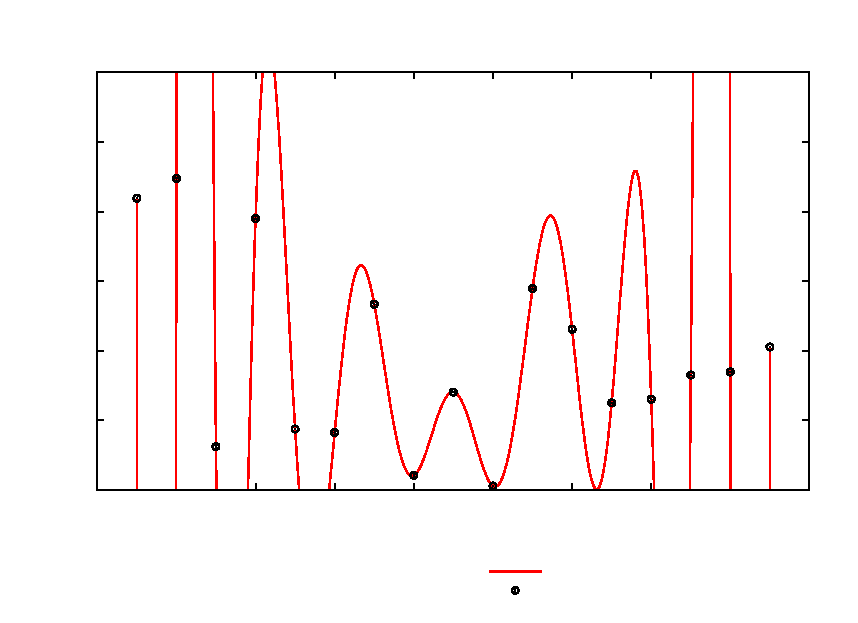
\includegraphics{./../LaTeX/graph/quest2-zoom}}%
    \gplfronttext
  \end{picture}%
\endgroup

	\caption{zoom para observar as oscilações}
	\label{fig:quest2-zoom}
	\end{subfigure}
	\caption{Gráficos da questão 2}
\end{figure}
\FloatBarrier




\begin{table}[!htp]
\centering
	\begin{tabular}{|l|l|}\hline
	n & $\alpha_{n}$ \\ \hline
			 0 &  178876.609375 \\ \hline 
		 1 &  -5959122.500000 \\ \hline 
		 2 &  85139872.000000 \\ \hline 
		 3 &  -703381504.000000 \\ \hline 
		 4 &  3801950720.000000 \\ \hline 
		 5 &  -14372312064.000000 \\ \hline 
		 6 &  39551909888.000000 \\ \hline 
		 7 &  -81234345984.000000 \\ \hline 
		 8 &  126366121984.000000 \\ \hline 
		 9 &  -149897789440.000000 \\ \hline 
		 10 &  135543185408.000000 \\ \hline 
		 11 &  -92683173888.000000 \\ \hline 
		 12 &  47087448064.000000 \\ \hline 
		 13 &  -17216391168.000000 \\ \hline 
		 14 &  4279737856.000000 \\ \hline 
		 15 &  -647252864.000000 \\ \hline 
		 16 &  44927628.000000 \\ \hline 
		 16 &  44927628.000000 \\ \hline 

	\end{tabular}
	\caption{Coeficientes de $y_{16}(t)$}
	\label{tab:quest2-X16}
\end{table}
